\documentclass{article}
\usepackage{longtable}

%\VignetteIndexEntry{C2C12}

\title{Analysis of C2C12 cell miRNA and mRNA expression data using the \textbf{miRNAmRNA} package}
\author{Maarten van Iterson}

\usepackage{Sweave}
\begin{document}

\maketitle

\section{minimal example}

Download target predictions manually from PITA, TargetScan and microCosm. Optionally construct parser for other prediction tools see ?addTable.


Construct the database and inspect its content.

\begin{Schunk}
\begin{Sinput}
> addTable(filePITA, tableName="pita", path=reultsDir, dbName=dbName, Org="Mm") 
> addTable(fileMicrocosm, tableName="microcosm", path=resultsDir, dbName=dbName, Org="Mm") 
> addTable(fileTargetScan, tableName="targetscan", path=resultsDir, dbName=dbName, Org="Mm") 
> dbInfo(resultsDir, dbName)
> dbHeadTable(resultsDir, dbName, "pita")
> dbHeadTable(resultsDir, dbName, "targetscan")
> dbHeadTable(resultsDir, dbName, "microcosm", n=10)
\end{Sinput}
\end{Schunk}

Download microRNA and mRNA expression data and perform some preprocessing steps such as identifier mapping.

\begin{Schunk}
\begin{Sinput}
> ##extract and process data
> library(GEOquery)
> miRNA <- getGEO(filename=file.path(dataDir, "expression_data", "GSE9449_series_matrix.txt.gz")) #also available from ArrayExpress E-GEOD-9449
> miFeature <- pData(featureData(miRNA))
> miExprs <- exprs(miRNA)
> colnames(miExprs) <- c("Prol", "Conf", "+1d", "+2d", "+4d")
> strwhite <- function(x)
+   {
+     x <- sub("^[[:blank:]]*", "", x, perl=TRUE) ##leading
+     x <- sub("[[:blank:]]*$", "", x, perl=TRUE) ##trailing
+     x
+   }
> extractID <- function(x)
+   {
+     y <- unlist(strsplit(x, ","))
+     idx <- sapply(y, grepl, pattern="mmu")
+     if(any(idx))
+       return(strwhite(y[idx]))
+     NA
+   }
> mirID <- sapply(as.character(miFeature$SPOT_ID), extractID, USE.NAMES=FALSE)
> rownames(miExprs) <- mirID
> miExprs <- miExprs[,-4] 
> miExprs <- miExprs[!is.na(rownames(miExprs)), ]
> miExprs <- miExprs[!duplicated(rownames(miExprs)),]
> ##some manual edits
> rownames(miExprs)[rownames(miExprs) == "mmu-miR-291a5p291b5p"] <- "mmu-miR-291a5p"
> rownames(miExprs)[rownames(miExprs) == "mmu-miR-133a133b"] <- "mmu-miR-133a"
> save(miExprs, file=file.path(resultsDir, "miExprs.RData"))
\end{Sinput}
\end{Schunk}

\begin{Schunk}
\begin{Sinput}
> mRNA <- getGEO(filename=file.path(dataDir, "expression_data", "GSE19968_series_matrix.txt.gz")) 
> mFeature <- pData(featureData(mRNA))
> mExprs <- exprs(mRNA)
> mExprs <- cbind(rowMeans(mExprs[,1:3]), rowMeans(mExprs[,4:6]), rowMeans(mExprs[,7:9]), rowMeans(mExprs[,10:12]))
> colnames(mExprs) <- c("Myoblast", "T0", "T24", "Myotube")
> mExprs <- mExprs[!duplicated(mFeature$GENE),,drop=FALSE] #extra calculation: remove all the mRNAs that map to the same Gene just using one transcript
> rownames(mExprs) <- mFeature$GENE[!duplicated(mFeature$GENE)]
> save(mExprs, file=file.path(resultsDir, "mExprs.RData"))
\end{Sinput}
\end{Schunk}

Run the integrated analysis.

\begin{Schunk}
\begin{Sinput}
> library(miRNAmRNA)
> dbName <- "mir.Mm.db"
> resultsDir <- "/home/mviterson/Documents/packages/miRNAmRNA"
> load(file.path(resultsDir, "mExprs.RData"))
> load(file.path(resultsDir, "miExprs.RData"))
> results <- rungt(mirs=rownames(miExprs), X=mExprs, Y=miExprs, path=resultsDir, dbName=dbName, tables=c("microcosm", "pita", "targetscan"), numOverlapping=3)
> save(results, file=file.path(resultsDir, "C2C12pairs.RData"))
\end{Sinput}
\end{Schunk}

\begin{Schunk}
\begin{Sinput}
> library(lattice)
> library(directlabels)
> resultsDir <- "/home/mviterson/Documents/packages/miRNAmRNA"
> load(file.path(resultsDir, "miExprs.RData"))
> load(file=file.path(resultsDir, "C2C12pairs.RData"))
> topMirs <- head(results$mirs, n=20)
> X <- miExprs[rownames(miExprs) %in% rownames(topMirs), ]
> data <- data.frame(miExpr = as.vector(X),
+                    Time =  rep(factor(colnames(X), levels = colnames(X), ordered=TRUE), each=nrow(X)),
+                    miRNA = gsub("mmu-", "", rep(rownames(X), ncol(X))))
> print(direct.label(xyplot(miExpr~Time, groups=miRNA, data, type=c("b", "g"), lwd=2, ylab=expression('Normalized '*log[2]*' ratio'),
+              scales = list(x = list(labels = colnames(X))))))
\end{Sinput}
\end{Schunk}
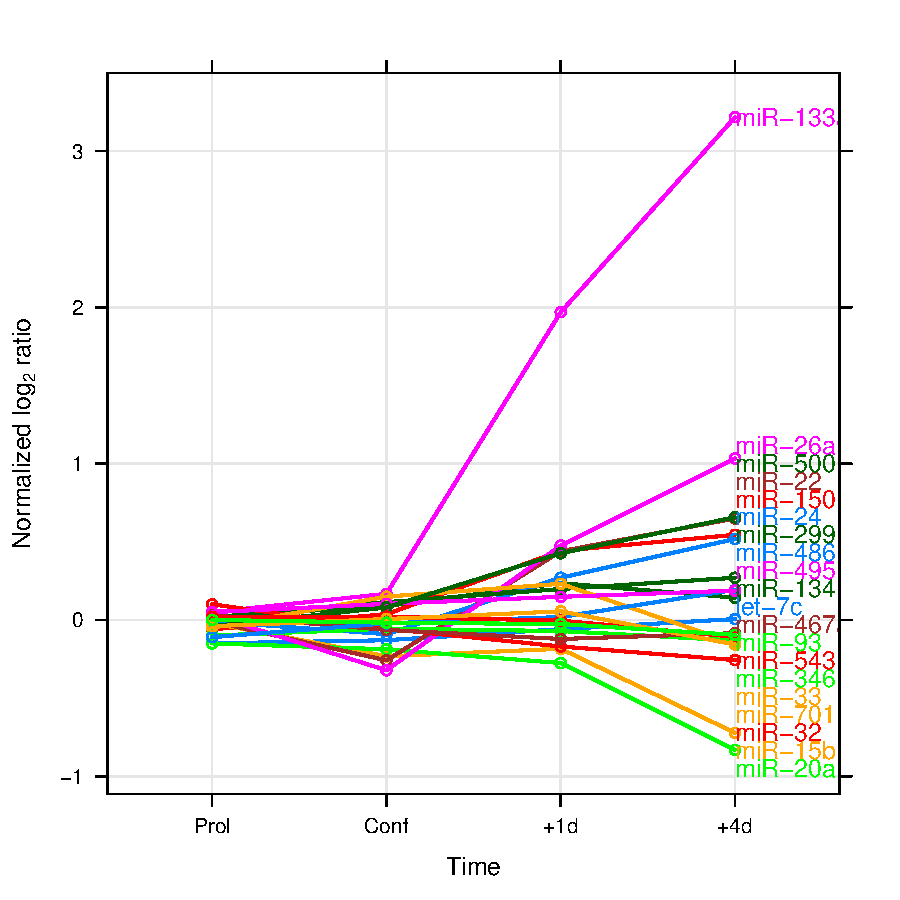
\includegraphics{C2C12-figure1}

\begin{Schunk}
\begin{Sinput}
> library(xtable)
> resultsDir <- "/home/mviterson/Documents/packages/miRNAmRNA"
> load(file=file.path(resultsDir, "C2C12pairs.RData"))
> topMirs <- head(results$mirs, n=20)
> topMiExprs <- miExprs[rownames(miExprs) %in% rownames(topMirs),c(1,4)]
> mirExprs <- topMiExprs[,1] < topMiExprs[,2]
> mirExprs[mirExprs==TRUE] <- "up"
> mirExprs[mirExprs==FALSE] <- "down"
> topMirs <- merge(topMirs, mirExprs, by="row.names")
> colnames(topMirs) <-  c("miRNA", "P-value", "\\# targets", "Regulation")
> xtable(topMirs[order(topMirs$'P-value'), ],
+        display=c("d", "s", "f", "d", "s"), digits= c(0, 0, 5, 0, 0),
+        caption="Overview of significant miRNA target sets with strict overlap between the three prediction tools TargetScan, MicroCosm and PITA.")
\end{Sinput}
% latex table generated in R 2.14.1 by xtable 1.7-0 package
% Wed Dec 19 12:11:38 2012
\begin{table}[ht]
\begin{center}
\begin{tabular}{rlrrl}
  \hline
 & miRNA & P-value & $\backslash$\# targets & Regulation \\ 
  \hline
3 & mmu-miR-134 & 0.00366 & 5 & up \\ 
  6 & mmu-miR-20a & 0.00677 & 134 & down \\ 
  17 & mmu-miR-500 & 0.01090 & 23 & up \\ 
  2 & mmu-miR-133a & 0.01230 & 49 & up \\ 
  1 & mmu-let-7c & 0.01614 & 86 & up \\ 
  8 & mmu-miR-24 & 0.02212 & 47 & up \\ 
  13 & mmu-miR-346 & 0.02681 & 4 & down \\ 
  20 & mmu-miR-93 & 0.03190 & 124 & down \\ 
  19 & mmu-miR-701 & 0.03250 & 1 & down \\ 
  10 & mmu-miR-299 & 0.03305 & 8 & up \\ 
  5 & mmu-miR-15b & 0.03308 & 100 & down \\ 
  15 & mmu-miR-486 & 0.03409 & 13 & up \\ 
  11 & mmu-miR-32 & 0.03616 & 120 & down \\ 
  9 & mmu-miR-26a & 0.03693 & 76 & up \\ 
  16 & mmu-miR-495 & 0.05060 & 48 & up \\ 
  14 & mmu-miR-467a & 0.05228 & 34 & down \\ 
  18 & mmu-miR-543 & 0.05705 & 55 & down \\ 
  12 & mmu-miR-33 & 0.06556 & 20 & down \\ 
  4 & mmu-miR-150 & 0.06703 & 17 & up \\ 
  7 & mmu-miR-22 & 0.07198 & 41 & up \\ 
   \hline
\end{tabular}
\caption{Overview of significant miRNA target sets with strict overlap between the three prediction tools TargetScan, MicroCosm and PITA.}
\end{center}
\end{table}\end{Schunk}



\begin{Schunk}
\begin{Sinput}
> print(xtable(mir22[,-c(4,5)],
+        display=c("d", "s", "f", "s"), digits=c(0,0,5,0),
+        caption="Overview of microRNA mmu-miR-22 targets with strict overlap between the three databases TargetScan, Microcosm and PITA."),
+        tabular.environment="longtable", floating=FALSE)
\end{Sinput}
% latex table generated in R 2.14.1 by xtable 1.7-0 package
% Wed Dec 19 12:11:38 2012
\begin{longtable}{rlrl}
  \hline
 & Symbol & Pvalue & Association \\ 
  \hline
83767 & Wasf1 & 0.00415 & neg. \\ 
  233902 & Fbxl19 & 0.07967 & neg. \\ 
  76932 & Arfip2 & 0.12357 & neg. \\ 
  19159 & Cyth3 & 0.13766 & neg. \\ 
  67771 & Arpc5 & 0.18739 & neg. \\ 
  14815 & Nr3c1 & 0.31383 & neg. \\ 
  17536 & Meis2 & 0.32297 & neg. \\ 
  22329 & Vcam1 & 0.34188 & neg. \\ 
  21345 & Tagln & 0.45586 & neg. \\ 
  16852 & Lgals1 & 0.47281 & neg. \\ 
  67074 & Mon2 & 0.51303 & neg. \\ 
  230596 & Prpf38a & 0.54665 & neg. \\ 
  108112 & Eif4ebp3 & 0.55761 & neg. \\ 
  67877 & Naa20 & 0.57213 & neg. \\ 
  231887 & Pdap1 & 0.66938 & neg. \\ 
  219094 & Khnyn & 0.76520 & neg. \\ 
  75770 & Brsk2 & 0.90336 & neg. \\ 
  12226 & Btg1 & 0.97314 & neg. \\ 
  12391 & Cav3 & 0.03830 & pos. \\ 
  67092 & Gatm & 0.05633 & pos. \\ 
  232087 & Mat2a & 0.06313 & pos. \\ 
  56323 & Dnajb5 & 0.12344 & pos. \\ 
  30948 & Bin1 & 0.14616 & pos. \\ 
  104263 & Kdm3a & 0.21728 & pos. \\ 
  66240 & Kcne1l & 0.36748 & pos. \\ 
  107271 & Yars & 0.36959 & pos. \\ 
  216850 & Kdm6b & 0.52230 & pos. \\ 
  27281 & Hrasls & 0.54816 & pos. \\ 
  70315 & Hdac8 & 0.54844 & pos. \\ 
  380916 & Lrch1 & 0.55348 & pos. \\ 
  234964 & Ccdc67 & 0.57421 & pos. \\ 
  229700 & Rbm15 & 0.58935 & pos. \\ 
  13831 & Epc1 & 0.60787 & pos. \\ 
  17257 & Mecp2 & 0.69782 & pos. \\ 
  276952 & Rasl10b & 0.75741 & pos. \\ 
  16918 & Mycl1 & 0.78415 & pos. \\ 
  18285 & Odf1 & 0.78714 & pos. \\ 
  245469 & Pdzd4 & 0.82422 & pos. \\ 
  239318 & Plcxd3 & 0.87587 & pos. \\ 
  56349 & Net1 & 0.96627 & pos. \\ 
  12978 & Csf1r & 0.97297 & pos. \\ 
   \hline
\hline
\caption{Overview of microRNA mmu-miR-22 targets with strict overlap between the three databases TargetScan, Microcosm and PITA.}
\end{longtable}\end{Schunk}
       
\begin{Schunk}
\begin{Sinput}
> print(xtable(mir133a[,-c(4,5)],
+        display=c("d", "s", "f", "s"), digits=c(0,0,5,0),
+        caption="Overview of microRNA mmu-miR-133a targets with strict overlap between the three databases TargetScan, Microcosm and PITA."),
+        tabular.environment="longtable", floating=FALSE)
\end{Sinput}
% latex table generated in R 2.14.1 by xtable 1.7-0 package
% Wed Dec 19 12:11:38 2012
\begin{longtable}{rlrl}
  \hline
 & Symbol & Pvalue & Association \\ 
  \hline
108013 & Celf4 & 0.00224 & neg. \\ 
  17300 & Foxc1 & 0.00895 & neg. \\ 
  13017 & Ctbp2 & 0.00962 & neg. \\ 
  29813 & Zfp385a & 0.01417 & neg. \\ 
  56195 & Ptbp2 & 0.02202 & neg. \\ 
  76932 & Arfip2 & 0.02642 & neg. \\ 
  56526 & Sept6 & 0.03019 & neg. \\ 
  23873 & Faim & 0.03089 & neg. \\ 
  19671 & Rce1 & 0.04030 & neg. \\ 
  13345 & Twist2 & 0.04046 & neg. \\ 
  19052 & Ppp2ca & 0.05338 & neg. \\ 
  13639 & Efna4 & 0.05490 & neg. \\ 
  70122 & Mllt3 & 0.07573 & neg. \\ 
  21873 & Tjp2 & 0.08822 & neg. \\ 
  223870 & Senp1 & 0.09540 & neg. \\ 
  13681 & Eif4a1 & 0.14082 & neg. \\ 
  17925 & Myo9b & 0.14631 & neg. \\ 
  66940 & Shisa5 & 0.14670 & neg. \\ 
  17886 & Myh9 & 0.14858 & neg. \\ 
  105522 & Ankrd28 & 0.18061 & neg. \\ 
  14573 & Gdnf & 0.18734 & neg. \\ 
  19053 & Ppp2cb & 0.19079 & neg. \\ 
  74442 & Sgms2 & 0.21377 & neg. \\ 
  83675 & Bicc1 & 0.22581 & neg. \\ 
  72587 & Pan3 & 0.26695 & neg. \\ 
  12757 & Clta & 0.28853 & neg. \\ 
  66500 & Slc30a7 & 0.39067 & neg. \\ 
  22218 & Sumo1 & 0.40243 & neg. \\ 
  66588 & Cmpk1 & 0.40671 & neg. \\ 
  217214 & Nags & 0.55364 & neg. \\ 
  69257 & Elf2 & 0.63642 & neg. \\ 
  76787 & Ppfia3 & 0.66704 & neg. \\ 
  242667 & Dlgap3 & 0.80598 & neg. \\ 
  224530 & Acat3 & 0.80903 & neg. \\ 
  16873 & Lhx5 & 0.86312 & neg. \\ 
  56389 & Stx5a & 0.86889 & neg. \\ 
  19272 & Ptprk & 0.00593 & pos. \\ 
  19228 & Pth1r & 0.12300 & pos. \\ 
  216190 & Appl2 & 0.35621 & pos. \\ 
  78593 & Nrip3 & 0.47936 & pos. \\ 
  243312 & Elfn1 & 0.48227 & pos. \\ 
  216549 & Aftph & 0.52637 & pos. \\ 
  14167 & Fgf12 & 0.54326 & pos. \\ 
  21854 & Timm17a & 0.57684 & pos. \\ 
  108071 & Grm5 & 0.82700 & pos. \\ 
  19277 & Ptpro & 0.87367 & pos. \\ 
  13803 & Enc1 & 0.93127 & pos. \\ 
  226896 & Tcfap2d & 0.99817 & pos. \\ 
  99326 & Garnl3 & 0.99828 & pos. \\ 
   \hline
\hline
\caption{Overview of microRNA mmu-miR-133a targets with strict overlap between the three databases TargetScan, Microcosm and PITA.}
\end{longtable}\end{Schunk}

\begin{Schunk}
\begin{Sinput}
> print(xtable(mir26a[,-c(4,5)],
+        display=c("d", "s", "f", "s"), digits=c(0,0,5,0),
+        caption="Overview of microRNA mmu-miR-26a targets with strict overlap between the three databases TargetScan, Microcosm and PITA."),
+        tabular.environment="longtable", floating=FALSE)
\end{Sinput}
% latex table generated in R 2.14.1 by xtable 1.7-0 package
% Wed Dec 19 12:11:38 2012
\begin{longtable}{rlrl}
  \hline
 & Symbol & Pvalue & Association \\ 
  \hline
230753 & Thrap3 & 0.00975 & neg. \\ 
  15402 & Hoxa5 & 0.01171 & neg. \\ 
  14163 & Fgd1 & 0.01818 & neg. \\ 
  18753 & Prkcd & 0.03200 & neg. \\ 
  59027 & Nampt & 0.03455 & neg. \\ 
  15234 & Hgf & 0.03738 & neg. \\ 
  233902 & Fbxl19 & 0.04957 & neg. \\ 
  18578 & Pde4b & 0.05925 & neg. \\ 
  68732 & Lrrc16a & 0.06011 & neg. \\ 
  23873 & Faim & 0.07397 & neg. \\ 
  264064 & Cdk8 & 0.08502 & neg. \\ 
  66197 & Cks2 & 0.09182 & neg. \\ 
  15446 & Hpgd & 0.13005 & neg. \\ 
  72549 & Reep4 & 0.18209 & neg. \\ 
  13836 & Epha2 & 0.18782 & neg. \\ 
  66980 & Zdhhc6 & 0.20504 & neg. \\ 
  52708 & Zfp410 & 0.22480 & neg. \\ 
  14056 & Ezh2 & 0.23016 & neg. \\ 
  16647 & Kpna2 & 0.23713 & neg. \\ 
  242466 & Zfp462 & 0.31819 & neg. \\ 
  233833 & Tnrc6a & 0.41264 & neg. \\ 
  12018 & Bak1 & 0.44428 & neg. \\ 
  235441 & Usp3 & 0.59153 & neg. \\ 
  217154 & Stac2 & 0.60107 & neg. \\ 
  13445 & Cdk2ap1 & 0.61613 & neg. \\ 
  66695 & Aspn & 0.69023 & neg. \\ 
  503610 & Zdhhc18 & 0.73335 & neg. \\ 
  77128 & A930001N09Rik & 0.78505 & neg. \\ 
  17532 & Mras & 0.89128 & neg. \\ 
  100019 & Mdn1 & 0.90387 & neg. \\ 
  232288 & Frmd4b & 0.01550 & pos. \\ 
  215814 & Ccdc28a & 0.02566 & pos. \\ 
  27402 & Pdhx & 0.04878 & pos. \\ 
  22057 & Tob1 & 0.04902 & pos. \\ 
  60613 & Kcnq4 & 0.05639 & pos. \\ 
  11535 & Adm & 0.05794 & pos. \\ 
  22652 & Mkrn3 & 0.06351 & pos. \\ 
  320538 & Ubn2 & 0.07083 & pos. \\ 
  18712 & Pim1 & 0.07706 & pos. \\ 
  234875 & Ttc13 & 0.09932 & pos. \\ 
  77044 & Arid2 & 0.10003 & pos. \\ 
  22065 & Trpc3 & 0.11484 & pos. \\ 
  30928 & Zfp238 & 0.12068 & pos. \\ 
  231290 & Slc10a4 & 0.14205 & pos. \\ 
  213753 & Zfp598 & 0.16269 & pos. \\ 
  229488 & Fam160a1 & 0.17340 & pos. \\ 
  320213 & Senp5 & 0.17368 & pos. \\ 
  231051 & Mll3 & 0.17701 & pos. \\ 
  74132 & Rnf6 & 0.18469 & pos. \\ 
  16650 & Kpna6 & 0.19984 & pos. \\ 
  231600 & Chfr & 0.22044 & pos. \\ 
  19212 & Pter & 0.23132 & pos. \\ 
  208177 & Phldb2 & 0.24115 & pos. \\ 
  99167 & Ssx2ip & 0.25254 & pos. \\ 
  76608 & Hectd3 & 0.31757 & pos. \\ 
  71795 & Pitpnc1 & 0.32328 & pos. \\ 
  19893 & Rpgr & 0.39004 & pos. \\ 
  227446 & 2310035C23Rik & 0.41007 & pos. \\ 
  228983 & Osbpl2 & 0.49724 & pos. \\ 
  74159 & Acbd5 & 0.49863 & pos. \\ 
  192285 & Phf21a & 0.51123 & pos. \\ 
  22241 & Ulk1 & 0.51187 & pos. \\ 
  17125 & Smad1 & 0.51643 & pos. \\ 
  225055 & Fbxo11 & 0.52365 & pos. \\ 
  238130 & Dock4 & 0.53668 & pos. \\ 
  106369 & Ypel1 & 0.53955 & pos. \\ 
  58242 & Nudt11 & 0.54688 & pos. \\ 
  71069 & Stox2 & 0.56330 & pos. \\ 
  14479 & Usp15 & 0.56787 & pos. \\ 
  67071 & Rps6ka6 & 0.64564 & pos. \\ 
  407823 & Baz2b & 0.67234 & pos. \\ 
  19266 & Ptprd & 0.68593 & pos. \\ 
  71673 & Rnf215 & 0.71344 & pos. \\ 
  13831 & Epc1 & 0.76169 & pos. \\ 
  269275 & Acvr1c & 0.76807 & pos. \\ 
  15112 & Hao1 & 0.95523 & pos. \\ 
   \hline
\hline
\caption{Overview of microRNA mmu-miR-26a targets with strict overlap between the three databases TargetScan, Microcosm and PITA.}
\end{longtable}\end{Schunk}


\end{document}

